\documentclass[letterpaper,11pt]{article}
\oddsidemargin -1.0cm \textwidth 17.5cm

\usepackage[utf8]{inputenc}
\usepackage[activeacute,spanish]{babel}
\usepackage{amsfonts,setspace}
\usepackage{amsmath}
\usepackage{amssymb, amsmath, amsthm}
\usepackage{comment}
\usepackage{float}
\usepackage{amssymb}
\usepackage{dsfont}
\usepackage{anysize}
\usepackage{multicol}
\usepackage{enumerate}
\usepackage{graphicx}
\usepackage[left=1.5cm,top=1.5cm,right=1.5cm, bottom=1.7cm]{geometry}
\setlength\headheight{1.5em} 
\usepackage{fancyhdr}
\usepackage{multicol}
\usepackage{hyperref}
\usepackage{wrapfig}
\usepackage{subcaption}
\pagestyle{fancy}
\fancyhf{}
\renewcommand{\labelenumi}{\normalsize\bfseries P\arabic{enumi}.}
\renewcommand{\labelenumii}{\normalsize\bfseries (\alph{enumii})}
\renewcommand{\labelenumiii}{\normalsize\bfseries \roman{enumiii})}

\begin{document}

\fancyhead[L]{\itshape{Facultad de Ciencias F\'isicas y Matem\'aticas}}
\fancyhead[R]{\itshape{Universidad de Chile}}

\begin{minipage}{11.5cm}
    \begin{flushleft}
        \hspace*{-0.6cm}\textbf{FI1100-6 Introducción a la Física Moderna}\\
        \hspace*{-0.6cm}\textbf{Profesor:} Diego Mardones\\
        \hspace*{-0.6cm}\textbf{Auxiliares:} Gabriel O\textsc{\char13}Ryan, Camila Sepúlveda, Alejandro Silva\\
        \hspace*{-0.6cm}\textbf{Ayudante:} Sebastián Vargas
    \end{flushleft}
\end{minipage}

\begin{picture}(1,1)
    \put(366, 10){
\includegraphics[scale=0.9]{Imágenes/logo/dfi-fcfm.pdf}}
\end{picture}

\begin{center}
	\LARGE\textbf{Auxiliar \#1:}\\
	\Large{Movimiento Armónico Simple}
\end{center}

\vspace{-1cm}
\begin{enumerate}\setlength{\itemsep}{0.4cm}

\rfoot[]{pág. \thepage}
\item[]

\item Una partícula realiza un MAS y su posición, dada por la expresión $x(t) = A\cos{(\omega t + \phi)}$, se muestra en el gráfico $x$ vs $t$ adjunto. Determine los valores $A$, $\omega$ y $\phi$ 
\begin{figure}[H]
    \centering
    \begin{subfigure}[t]{0.49\linewidth}
        \centering
        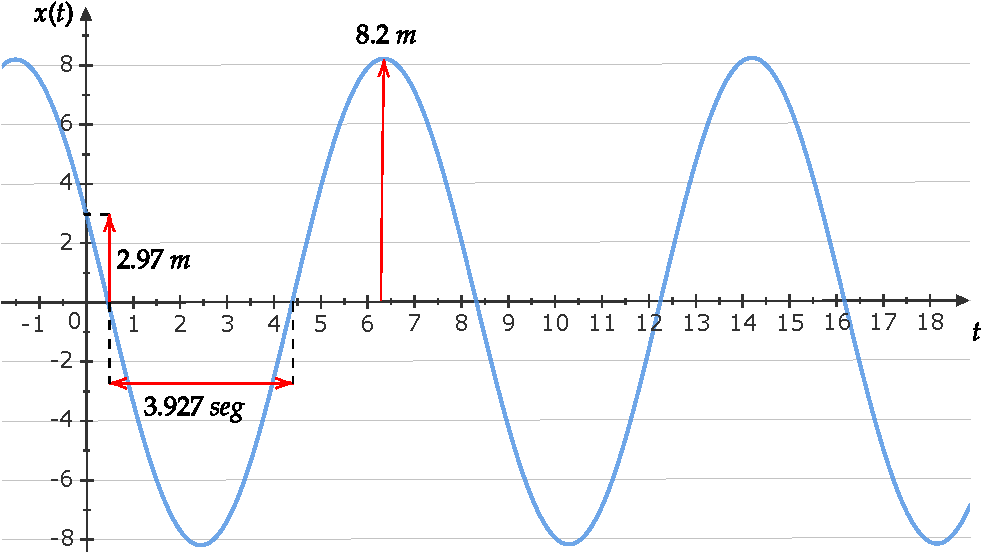
\includegraphics[width=\linewidth]{Imágenes/aux01/grafico.pdf}
    \end{subfigure}
\end{figure}
\item Un resorte de constante elástica $k$ cuelga verticalmente de un soporte. En su extremo inferior (que se encuentra a una distancia $\ell_0$ del techo) se engancha una masa $m$ que se suelta desde el reposo en el instante $t=0$. La masa comenzará a oscilar en torno a un nuevo punto de equilibro $x_0$.
    \begin{enumerate}
        \item Encuentre el nuevo punto de equilibrio $x_0$
        \item Determine el periodo de la oscilación de la masa $m$ en torno a $x_0$
        \item Determine la energía cinética y la energía potencial en función del tiempo
        \item ¿Cuál será la velocidad máxima que llegará a tener la masa $m$ mientras oscila?
    \end{enumerate}

\begin{figure}[H]
    \centering
    \begin{subfigure}[t]{0.49\linewidth}
        \centering
        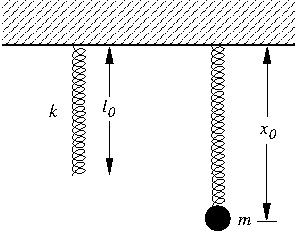
\includegraphics[width=0.55\linewidth]{Imágenes/aux01/resorte-techo.pdf}
        \caption*{Figura P2}
    \end{subfigure}
    \begin{subfigure}[t]{0.49\linewidth}
        \centering
        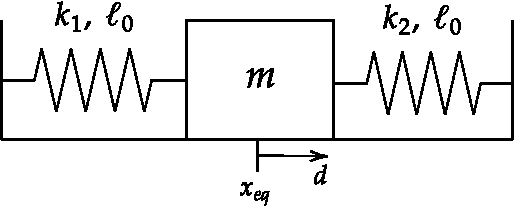
\includegraphics[width=0.7\linewidth]{Imágenes/aux01/dosresortes.pdf}
        \caption*{Figura P3}
    \end{subfigure}
\end{figure}
\item Una masa $m$ descansa sobre una superficie lisa horizontal unida a dos resortes de constantes $k_1$ y $k_2$, ambos de largo natural $\ell_0$, que inicialmente no tienen deformación alguna. Si desde la posición de equilibrio se perturba una distancia $d$ hacia la derecha y se suelta, determine el periodo de oscilación y la ecuación de movimiento.
\end{enumerate}
\end{document}